% Editable native annotations around unchanged verified IDE photographs.
\par
\begin{figure}[htbp]
  \centering
  \sbox0{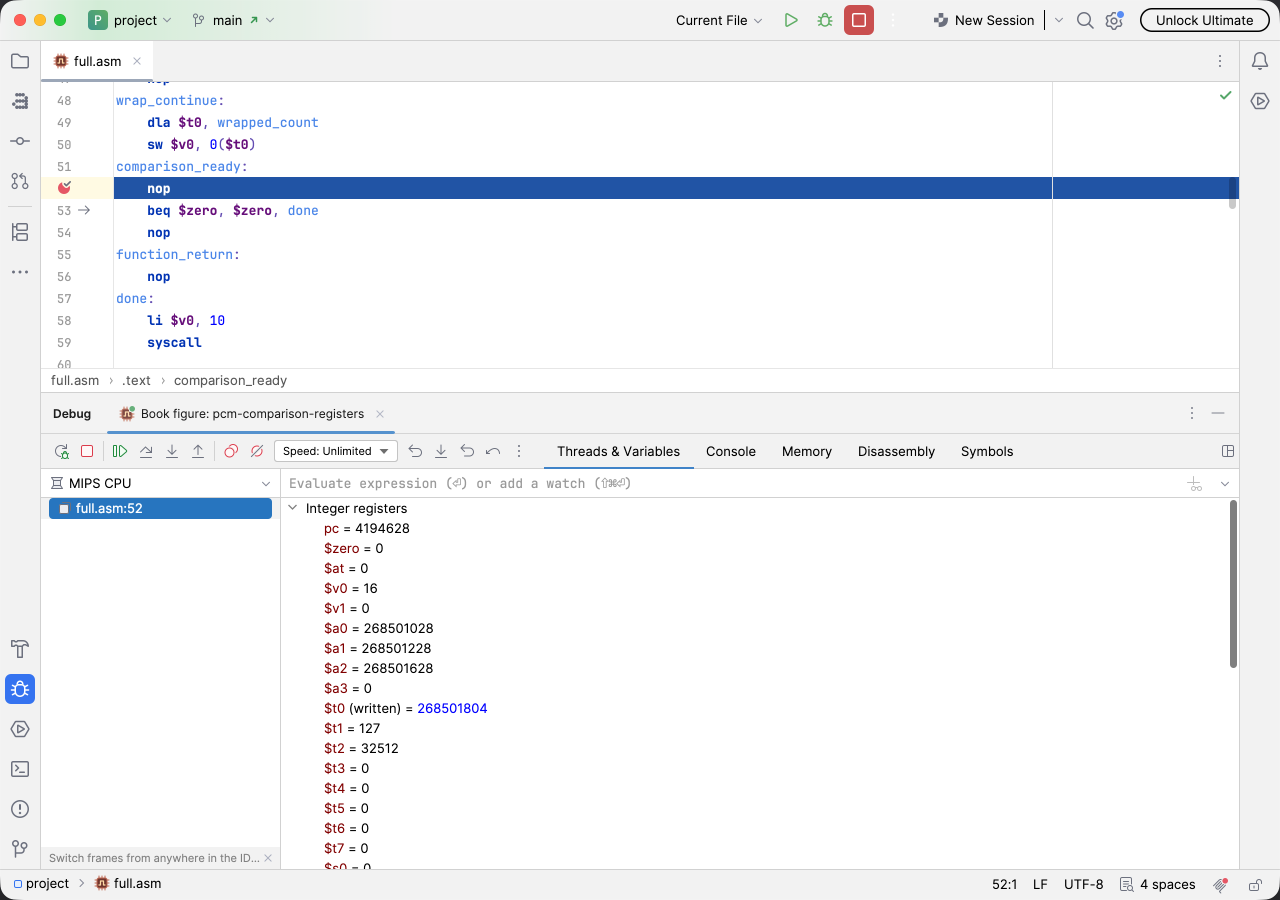
\includegraphics[artifact]{packages/020-pcm-mixing/captures/f03/registers.png}}
  \sbox2{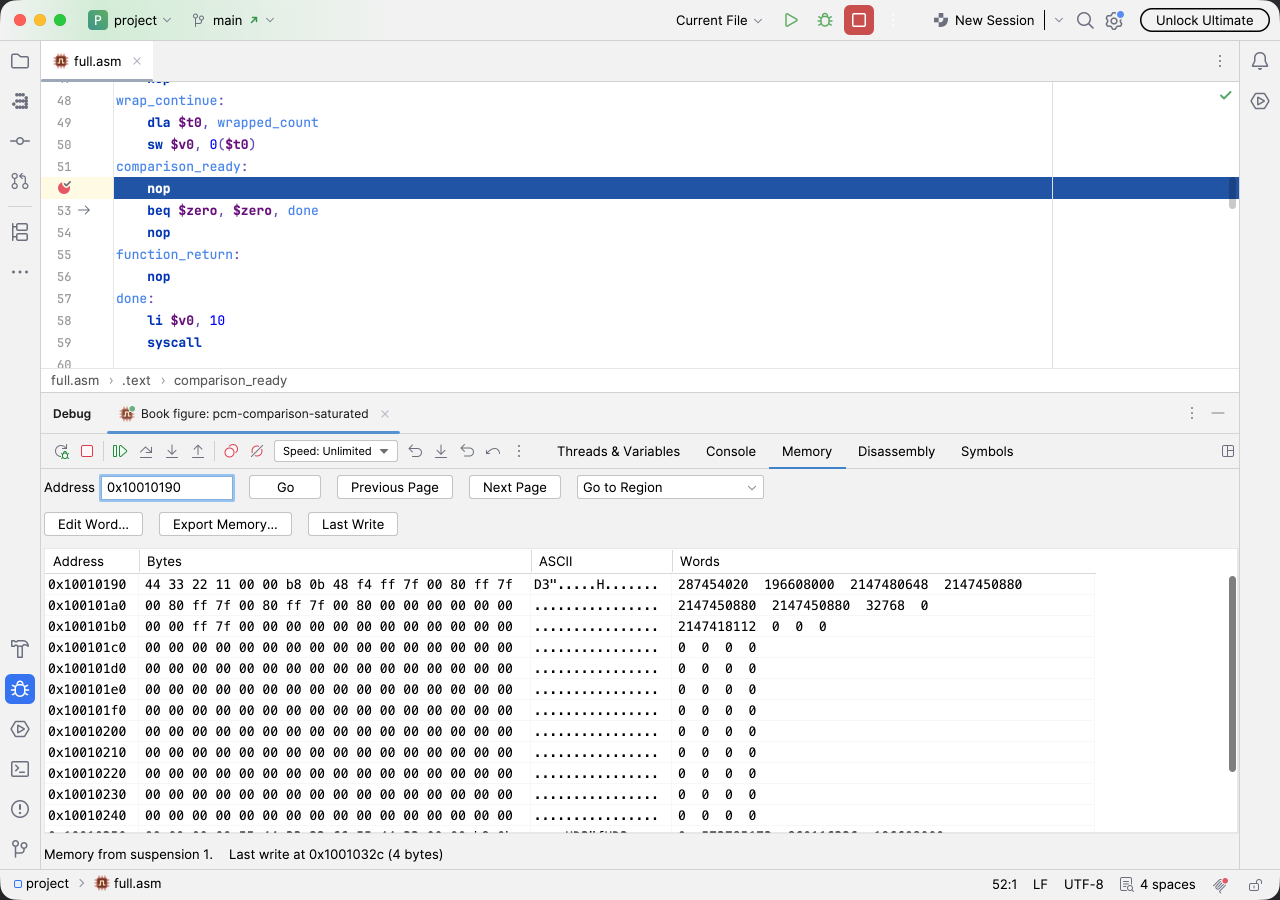
\includegraphics[artifact]{packages/020-pcm-mixing/captures/f03/saturated.png}}
  \sbox4{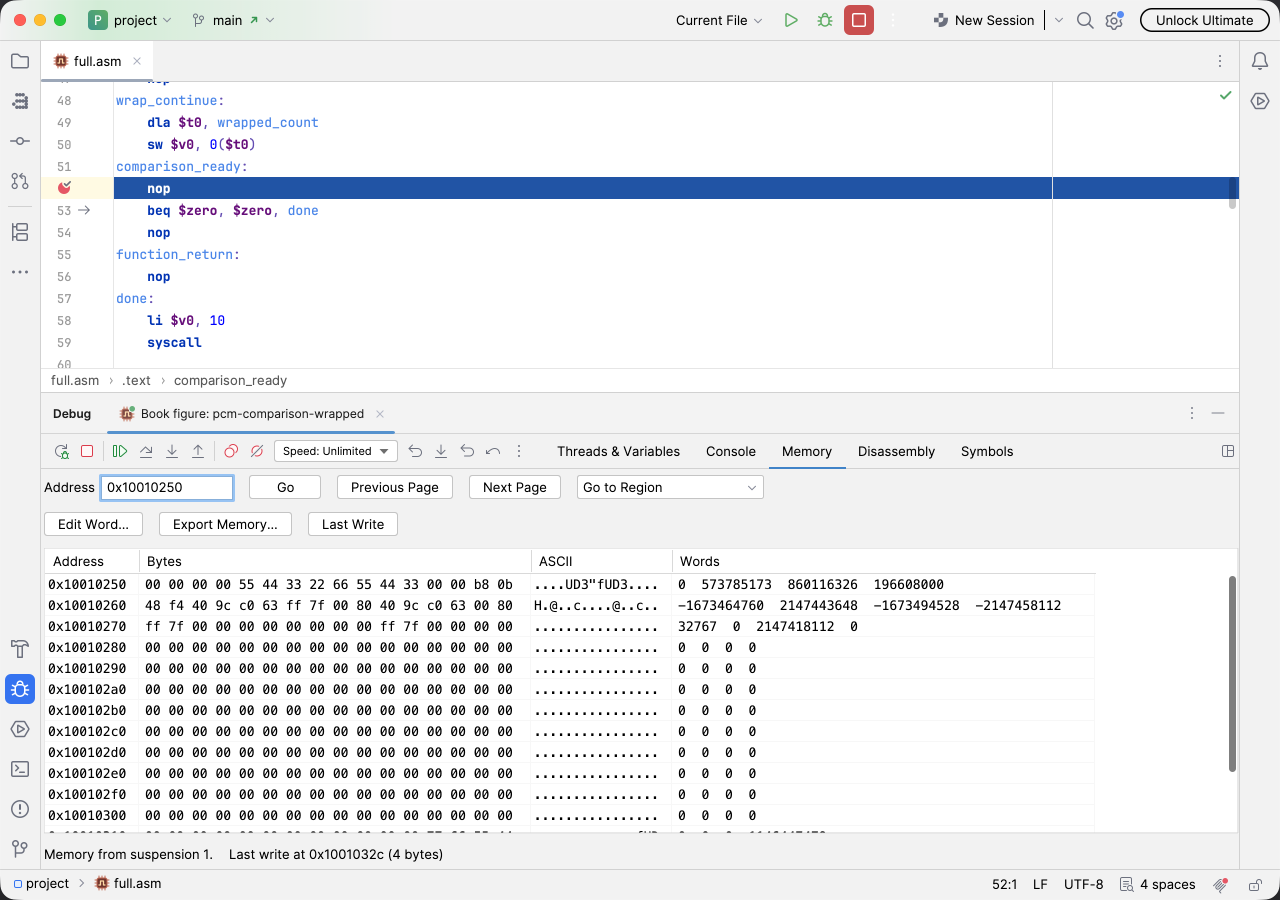
\includegraphics[artifact]{packages/020-pcm-mixing/captures/f03/wrapped.png}}
  \sbox6{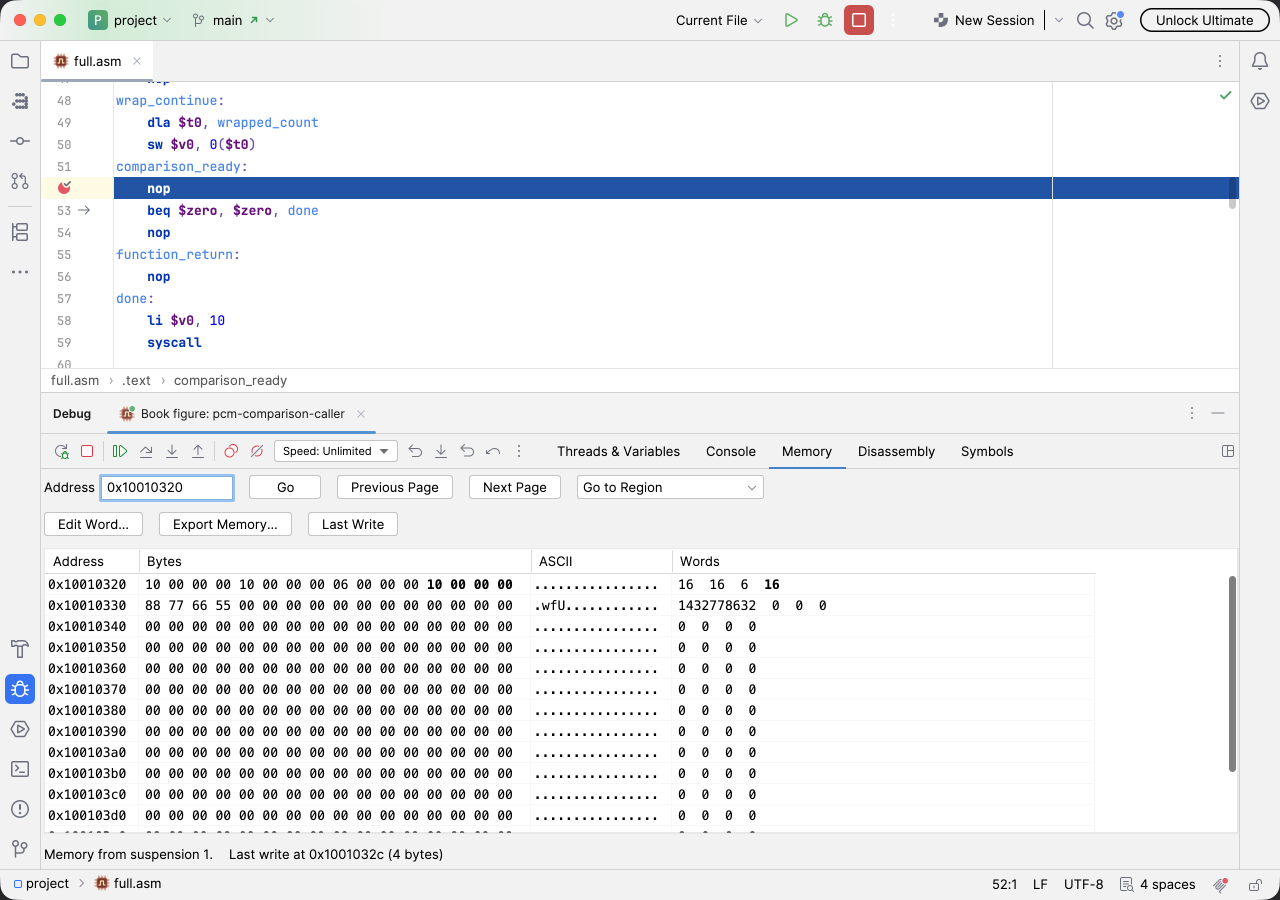
\includegraphics[artifact]{packages/020-pcm-mixing/captures/f03/caller.png}}
  \edef\MARSpcmcomparisonsourceLeft{\the\dimexpr0.036718750\wd0\relax}
  \edef\MARSpcmcomparisonsourceBottom{\the\dimexpr0.774444444\ht0\relax}
  \edef\MARSpcmcomparisonsourceRight{\the\dimexpr0.713281250\wd0\relax}
  \edef\MARSpcmcomparisonsourceTop{\the\dimexpr0.170000000\ht0\relax}
  \edef\MARSpcmcomparisonregistersLeft{\the\dimexpr0.246093750\wd0\relax}
  \edef\MARSpcmcomparisonregistersBottom{\the\dimexpr0.312222222\ht0\relax}
  \edef\MARSpcmcomparisonregistersRight{\the\dimexpr0.553906250\wd0\relax}
  \edef\MARSpcmcomparisonregistersTop{\the\dimexpr0.640000000\ht0\relax}
  \edef\MARSpcmcomparisonsaturatedLeft{\the\dimexpr0.034375000\wd2\relax}
  \edef\MARSpcmcomparisonsaturatedBottom{\the\dimexpr0.287777778\ht2\relax}
  \edef\MARSpcmcomparisonsaturatedRight{\the\dimexpr0.584375000\wd2\relax}
  \edef\MARSpcmcomparisonsaturatedTop{\the\dimexpr0.608888889\ht2\relax}
  \edef\MARSpcmcomparisonwrappedLeft{\the\dimexpr0.034375000\wd4\relax}
  \edef\MARSpcmcomparisonwrappedBottom{\the\dimexpr0.287777778\ht4\relax}
  \edef\MARSpcmcomparisonwrappedRight{\the\dimexpr0.584375000\wd4\relax}
  \edef\MARSpcmcomparisonwrappedTop{\the\dimexpr0.608888889\ht4\relax}
  \edef\MARSpcmcomparisoncallerLeft{\the\dimexpr0.034375000\wd6\relax}
  \edef\MARSpcmcomparisoncallerBottom{\the\dimexpr0.334444444\ht6\relax}
  \edef\MARSpcmcomparisoncallerRight{\the\dimexpr0.584375000\wd6\relax}
  \edef\MARSpcmcomparisoncallerTop{\the\dimexpr0.608888889\ht6\relax}
  \begin{tikzpicture}[alt={Five annotated panels at comparison_ready show current returns sixteen and zero, both complete 32-byte output slices, and caller words sixteen,sixteen,six,sixteen. Saturated and wrapping values agree for representable sums and differ for the six overflow cases. Input and guards remain unchanged; the later exit service has not executed.}]
    \node[anchor=north west,inner sep=0,font=\small\bfseries] (source-title) at (6mm,0) {Next instruction at this boundary};
    \node[anchor=north west,inner sep=0] (source) at ([yshift=-1mm]source-title.south west) {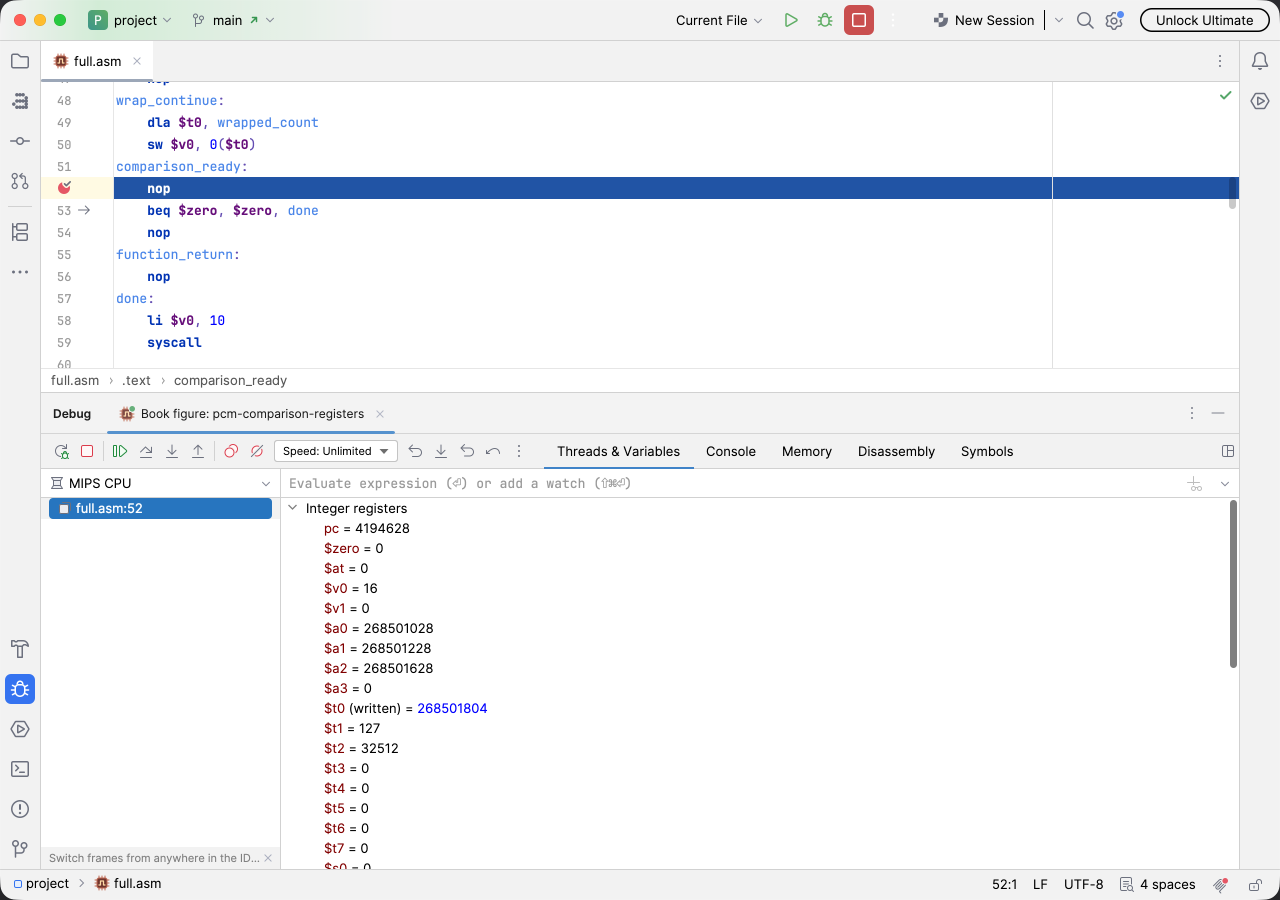
\includegraphics[width=0.54\linewidth,artifact,trim={\MARSpcmcomparisonsourceLeft{} \MARSpcmcomparisonsourceBottom{} \MARSpcmcomparisonsourceRight{} \MARSpcmcomparisonsourceTop{}},clip]{packages/020-pcm-mixing/captures/f03/registers.png}};
    \begin{scope}[shift={(source.south west)},x={($(source.south east)-(source.south west)$)},y={($(source.north west)-(source.south west)$)}]
      \draw[black,line width=0.7pt] (0.215625000,0.080000000) rectangle (0.384375000,0.520000000);
      \node[draw=black,fill=white,circle,inner sep=1.5pt,font=\footnotesize] at ($(0.215625000,0.520000000)+(-3mm,0)$) {1};
    \end{scope}
    \node[anchor=north west,inner sep=0,font=\small\bfseries] (registers-title) at (0.58\linewidth,0 |- source-title.north) {Current return values};
    \node[anchor=north west,inner sep=0] (registers) at ([yshift=-1mm]registers-title.south west) {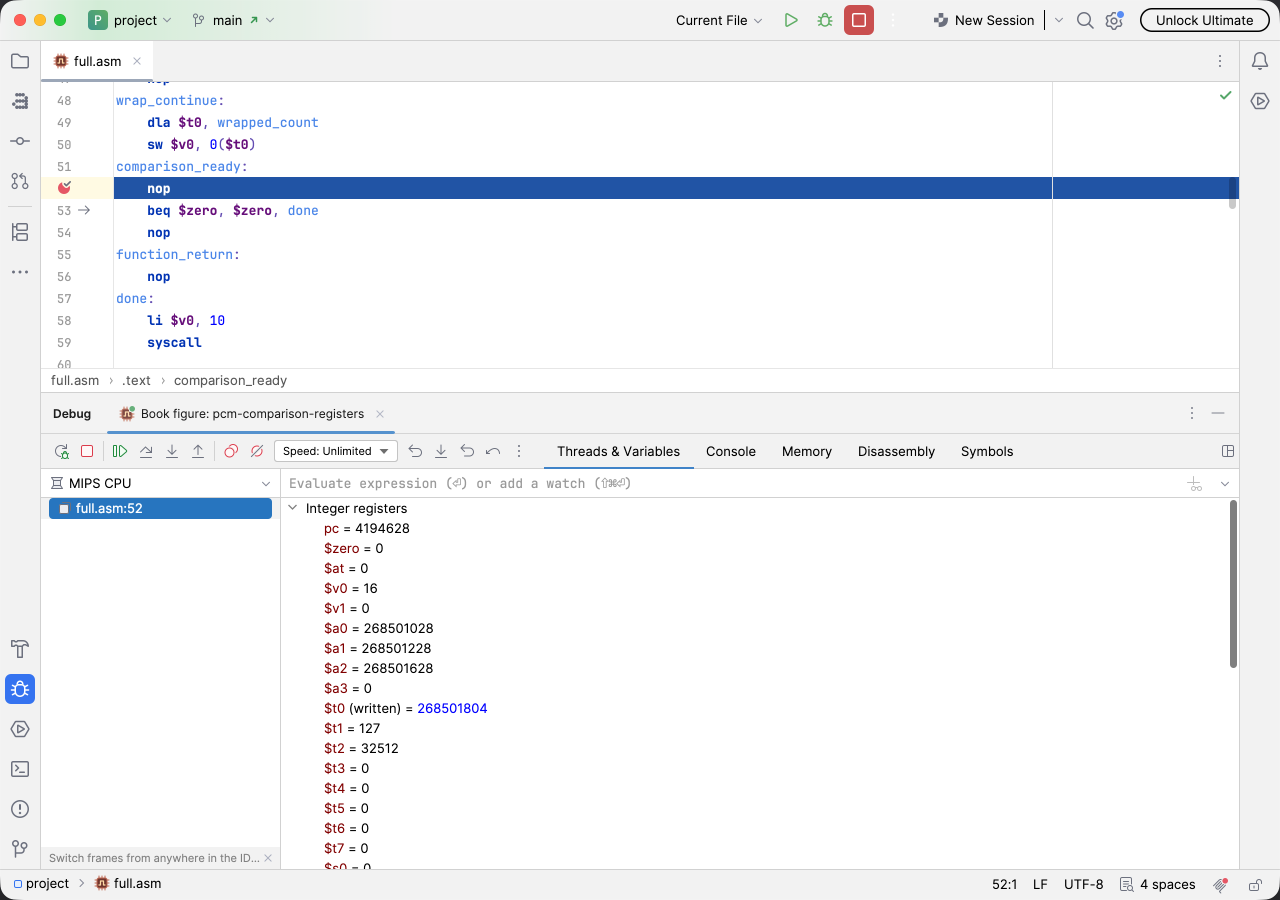
\includegraphics[width=0.42\linewidth,artifact,trim={\MARSpcmcomparisonregistersLeft{} \MARSpcmcomparisonregistersBottom{} \MARSpcmcomparisonregistersRight{} \MARSpcmcomparisonregistersTop{}},clip]{packages/020-pcm-mixing/captures/f03/registers.png}};
    \begin{scope}[shift={(registers.south west)},x={($(registers.south east)-(registers.south west)$)},y={($(registers.north west)-(registers.south west)$)}]
      \draw[black,line width=0.7pt] (0.023437500,0.023255814) rectangle (0.250000000,0.953488372);
      \node[draw=black,fill=white,circle,inner sep=1.5pt,font=\footnotesize] at ($(0.023437500,0.953488372)+(-3mm,0)$) {2};
    \end{scope}
    \node[anchor=north west,inner sep=0,font=\small\bfseries] (saturated-title) at ([yshift=-1mm]source.south west) {Signed saturated samples};
    \node[anchor=north west,inner sep=0] (saturated) at ([yshift=-1mm]saturated-title.south west) {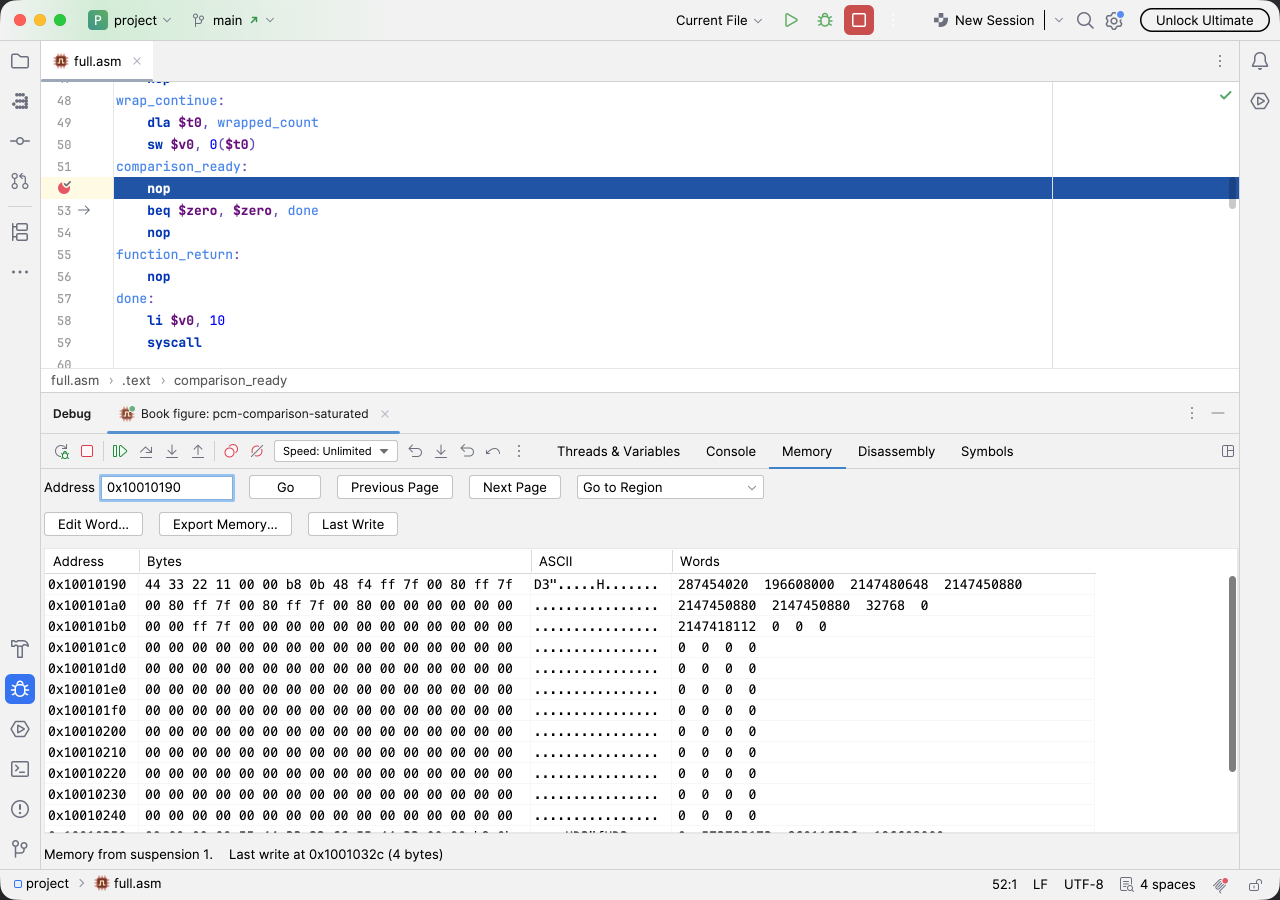
\includegraphics[width=0.84\linewidth,artifact,trim={\MARSpcmcomparisonsaturatedLeft{} \MARSpcmcomparisonsaturatedBottom{} \MARSpcmcomparisonsaturatedRight{} \MARSpcmcomparisonsaturatedTop{}},clip]{packages/020-pcm-mixing/captures/f03/saturated.png}};
    \begin{scope}[shift={(saturated.south west)},x={($(saturated.south east)-(saturated.south west)$)},y={($(saturated.north west)-(saturated.south west)$)}]
      \draw[black,line width=0.7pt] (0.194672131,0.043010753) rectangle (0.997950820,0.720430108);
      \node[draw=black,fill=white,circle,inner sep=1.5pt,font=\footnotesize] at ($(0,0.720430108)+(-3mm,0)$) {3};
    \end{scope}
    \node[anchor=north west,inner sep=0,font=\small\bfseries] (wrapped-title) at ([yshift=-1mm]saturated.south west) {Signed wrapping samples};
    \node[anchor=north west,inner sep=0] (wrapped) at ([yshift=-1mm]wrapped-title.south west) {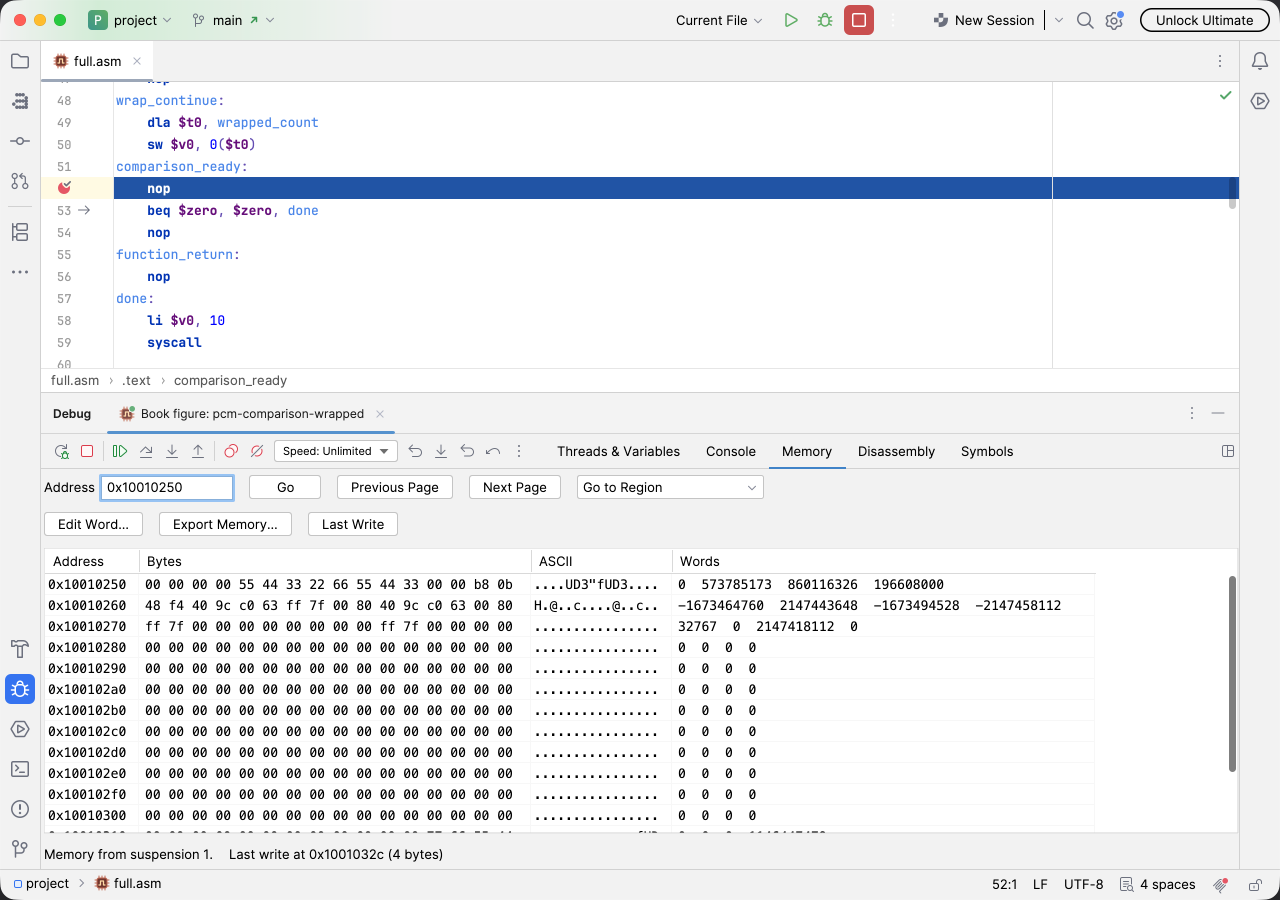
\includegraphics[width=0.84\linewidth,artifact,trim={\MARSpcmcomparisonwrappedLeft{} \MARSpcmcomparisonwrappedBottom{} \MARSpcmcomparisonwrappedRight{} \MARSpcmcomparisonwrappedTop{}},clip]{packages/020-pcm-mixing/captures/f03/wrapped.png}};
    \begin{scope}[shift={(wrapped.south west)},x={($(wrapped.south east)-(wrapped.south west)$)},y={($(wrapped.north west)-(wrapped.south west)$)}]
      \draw[black,line width=0.7pt] (0.194672131,0.043010753) rectangle (0.997950820,0.720430108);
      \node[draw=black,fill=white,circle,inner sep=1.5pt,font=\footnotesize] at ($(0,0.720430108)+(-3mm,0)$) {4};
    \end{scope}
    \node[anchor=north west,inner sep=0,font=\small\bfseries] (caller-title) at ([yshift=-1mm]wrapped.south west) {Count and saved caller results};
    \node[anchor=north west,inner sep=0] (caller) at ([yshift=-1mm]caller-title.south west) {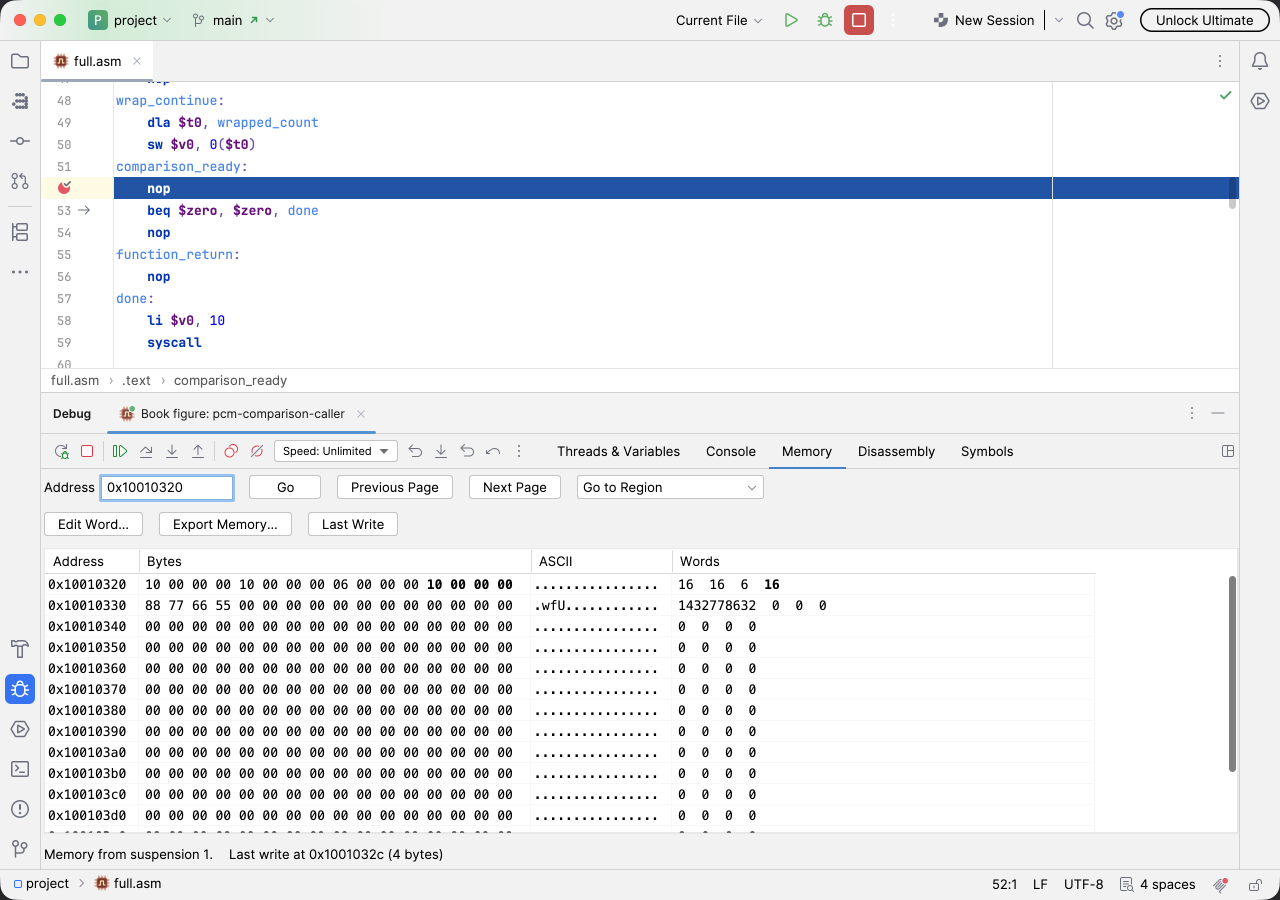
\includegraphics[width=0.84\linewidth,artifact,trim={\MARSpcmcomparisoncallerLeft{} \MARSpcmcomparisoncallerBottom{} \MARSpcmcomparisoncallerRight{} \MARSpcmcomparisoncallerTop{}},clip]{packages/020-pcm-mixing/captures/f03/caller.png}};
    \begin{scope}[shift={(caller.south west)},x={($(caller.south east)-(caller.south west)$)},y={($(caller.north west)-(caller.south west)$)}]
      \draw[black,line width=0.7pt] (0.194672131,0.078431373) rectangle (0.997950820,0.490196078);
      \node[draw=black,fill=white,circle,inner sep=1.5pt,font=\footnotesize] at ($(0,0.490196078)+(-3mm,0)$) {5};
    \end{scope}
  \end{tikzpicture}
  \par\smallskip
  \begin{minipage}{\linewidth}
    \small
    \begin{enumerate}
      \setlength{\itemsep}{2pt}
            \setlength{\parsep}{0pt}
      \item The blue \texttt{nop} at \texttt{comparison\_ready} follows the caller\textquotesingle s last result store. Both calls and all three publications are complete. This boundary is suitable for comparing the two buffers and their saved metadata together.
      \item The registers still hold the wrapping return, \texttt{\$v0 = 16} and \texttt{\$v1 = 0}. The saved \texttt{clipped} word carries the saturating result. Exit later reuses \texttt{v0} for a service number, so inspect the named boundary before termination.
      \item The saturated slice at \texttt{0x10010194} contains sixteen signed halfwords. Its last two values are 0 and 32767. Some samples land exactly on an endpoint; only the six sums outside the range incremented the clipping result.
      \item The wrapping slice at \texttt{0x1001025c} contains the same number of halfwords. It agrees with saturation for representable sums and differs for the six overflow cases. Read each low-byte-first pair as a signed sample. The two routines use the same source samples and apply different output rules.
      \item The caller row is now 16, 16, 6, 16: requested count, saturating processed count, clipped count and wrapping processed count. Input arrays and guards remain unchanged. The complete byte and access histories also check output suffixes beyond these sixteen samples.
    \end{enumerate}
  \end{minipage}
  \caption{The completed comparison preserves six clipped samples beside sixteen wrapping samples.}
  \label{capture:020-pcm-mixing-f03}
  \label{pcm-f03}
\end{figure}
\par
